
\documentclass[a4paper,singleside,12pt]{report} % Uncomment this for single side pdf.
%\documentclass[a4paper,twoside,12pt]{report} % Uncomment this for printing.

\usepackage{ai_bo_thesis}
\usepackage[english]{babel}
\usepackage[T1]{fontenc}
\usepackage{lmodern}


\usepackage[backend=biber,style=trad-plain, sorting=nty,firstinits=true]{biblatex}
\addbibresource{biblio.bib}

\setmainfont{Times New Roman}
\begin{document}
	
	\title{Towards sequential problem solving in ACT-R: a case study of TANGRAM}
	\topic{cognitive Architecture}
	\candidate{Giacomo Zamprogno}
	\supervisor{Prof. Giuseppe Di Pellegrino}
	\cosupervisor{co-supervisor} % One co-supervisor.
	%\cosupervisors{} % More than one co-supervisor.
	\academicyear{2021-2022}
	\session{1st}

	\frontispiece 
	\dedication{+retrieval> \\ ISA dedication \\ NAME tbd \\ REASON tbd}
	\toc
	\figstoc
	\tablestoc
	\begintext
	
	\chapter{Introduction}
    \textit{Where I describe cognitive modelling and its applications, and the specific case study
    of the tangram in the context manufacturing and tutoring}
	
	What is cognitive modelling? Why how does it relate to AI and why is it of interest at airbus?
	MAYBE the reserch group at airbus The idea of the project
	\section{Tangram}
	The tangram is an ancient Chinese puzzle in which seven pieces, also called \textit{tans} are
	obtained from an original square.\\
	The most common tans, also used in this work, consist of 5 square triangles (2 small, 1 medium
	and 2 large), 1 square and 1 parallelogram, their dimension is shown in Figure \ref{fig:tans}
	.\\
	\begin{figure}[h]
		\centering
		
\includegraphics{pictures/tan.png}
		\caption[]{Most commond tans and starting position}
		\label{fig:tans}
	\end{figure}
	Usually players are presented with an homogeneous silhouette, likely in the shape of some
	stylized figure, and are asked to reproduce the pattern by using all the tans, without
	overlap.\\
	Besides the interest among puzzle-solvers, a number of works has been studying its applications
	in the teaching fields, where its nature as a fairly complex game can help children to develop
	geometric and communicative skills[citation to some papers might be needed here].\\
	In the context of cognitive modelling, the tangram can be seen as an abstraction for a set of
	different sequential problem solving tasks. The fact that the field is still at the early stages
	of development, studying a simpler puzzle and how humans approach its solution might provide
	initial insights about various types of assembling processes, in an attempt to create machines
	more capable to interpret and adapt to human actions in an explainable and rule-based way. 	
    
    
    \chapter{Related Works}
    \textit{Where I quickly go throught the available Literature, describe ACT-R and its functioning
	and analyze the various approaches for tangram solving}
	
	\section{Cogntive modelling of puzzles}
	Despite their nature and potential as an abstraction for more sophisticated sequential problem
	solving tasks, the applicaions of cognitive modelling to puzzles are still at an early stage.\\
	Rosenberg et al. \cite{social-robot} coupled cognitive architectures and the tangram puzzle	in
	order to model the curiosity aspect of a social robot, but the actual solution of the puzzle was
	implemented with a connectionist approach and the cognitive aspect was focused on the social
	interaction and artificial curiosity modelling. Gentile and Lieto \cite{GENTILE20221} instead
	used ACT-R in order to model the role of mental rotation applied to the task of the
	Tetris\textsuperscript{TM} video-game, based on the previous work of Shepard and
	Metzler \cite{shepard1971mental}, providing introductory results and a functioning model for the
	mental rotation process.
	\section{Tangram}
	As mentioned, cognitive-modelling specific literature regarding the tangram is extremely
	limited. Nonetheless, previous works in the fields of computer science, neuroscience and cognitive psychology
	can be seen as an interesting starting baseline for the modelling process. \\Among the
	computational approaches, Deutsch and Hayes \cite{heuristic} originally suggested a heuristic
	solution based on extending the lines inside the silhouette and matching the edges of the tans
	with the prolonged lines; they intersetingly suggest an heuristic approach based on different
	types of matching, distinguishing between a direct matching type, where all the sides perfectly
	match, and a partial matching type, where only part of the edges match with the lines or their
	extensions. While possibly tangent to some cognitive processes at a higher level, the strictly
	geometrical nature of their solving algorithm and especially the complex evaluation of the lines
	extensions reduce its applicability in the current architecture.\\
	During the advent of machine learning, Oflazer \cite{Oflazer1993SolvingTP} used a Boltzmann
	Machine, where each neuron represented a possible positioning of one piece, and was fed with
	excitatory input from the outline constraints and inhibitory input from the conflicting
	configurations. The main limit of the approach is that the authors only tackle \textit{grid
	tangrams}, where each corner of a placed tan must be coincident with a point in an equally
	spaced grid. This in turn largely limits the allowed rotations for the pieces and thus its
	applicability, even at a knwoledge representation level, when dealing with less constrained
	puzzles as the irrational length of edges would be impossible to tackle using the grid. \\
	The work from Hu, Lam and Yuan \cite{Hu2019EffectiveCO} on neural activity during the tangram
	task suggests a possible direction to take in order to reproduce human behaviour. The authors
	monitored the fronto-paretal area during the puzzle solution, and propose that trial and error
	strategies might be prevalent instead of inductive reasoning. In this case, the need for
	forward reasoning mechanisms in the model might be reduced in favour of an insight based
	approach. 
	
	\section{ACT-R}

    
	
	\chapter{Experimental scenario}
    In collaboration with the Technical University of Berlin (TUB) an experiment was developed and
    performed in order to obtain the training and test sets.\\
	The participants were recruited among the students of the TUB, and two experiment sessions were
	held at different dates, with different participants, for a total of [waiting for test set].
	Participants signed an informed consent for the usage of the gathered data and were compensated
	with [which model?] miniatures provided by the company. Each participant was presented with a
	virtual implementation of the tangram game, including 4 puzzles [cite figure]. After an inital
	explanation of the controls, each participant was required to tackle the solution of the
	puzzles, which were always shown in the same order. There was no time limit, and at any moment
	the \textit{NEXT} button was available, so that the player could give up on the specific tangram
	and move to the next one. It must be noted that while backtracking was possible during the
	solution of the single task, once the button was pressed the solution was submitted and no
	option to go back was available.\\
	Between each problem, the participants were asked to complete a NASA evaluation form, and at the
	end of the trial they provided a general feedback. \\
	In addition to this, the screen recording and application logs, including data regarding times,
	piece action types (rotation, movement) and piece positioning were stored for the analysis. \\
	During the first trial set, 31 participants (17 males, 14 females) took part to the experiment;
	they all had an academic background, a large majority of them being from engineering or human
	factors studies. \\
	These first players composed the training set.
    
	
	\chapter{Data Analysis and Hypothesis}
    Where I qualitatively and quantitatively analyze the available data, provide figures and
    introduce the leading Hypothesis that the model will try to explain
    
	
	\chapter{Model description}
    
	The agent model consists of multiple sub-components and a coordinator which handles their
	interaction. The components are relatively distinct and provide the various functionalities of
	the system: the \textit{application} module creates and updates the experimental window, the
	\textit{landmark extractor} module implements the visual system and extracts "plausible" placements
	of the tans in the current state, the ACT-R module performs the main reasoning task and decides
	the next action.\\
    In principle, it would be possible to create and run an experimental setting entirely within the ACT-R
	context. In the specific case of the project, however, the available data were strictly
	dependent on the implementation of the experimental window: the coordinates for the placements
	of the tans were expressed with respect to the application window, and the tans themselves were
	defined as shapes within the framework. Reproducing the setting purely in ACT-R would likely
	have caused loss of precision in the shapes and coordinates definition, besides an additional
	overhead due to the lack of established methods for complex image manipulation: the creation an
	interfacing system was then preferred.\\
    
    \section{Experiment window}
	The applicaion window during the experiment was derived by an existing Tangram demo application
	[shall i cite? it comes from "tangram4kids"] and included interactive features which allowed the
	users to manipulate and move the tans. While such features were not required in the developed
	model, as no simulation of motor functions was planned, most of the data gathered during the
	experimental sessions was framed in the context of the application. As a result, a similar
	window was mantained for better corrspondence, and the model runs on a lighter adaptation of the
	code, providing just two main functionalities: it updates the window to represent the current state, and it
	captures the window screen so that it can be forwared to the visual system for processing.


    \section{Visual system}
    The agent's visual system was implemented in order to be "cognitively inspired" from the
    hierarchical structure of the human's visual system. Given the strictly geometrical nature of
    the puzzle, and the fact that \textit{second layer neurons} [need the proper name and citation]
    fire when matching certain oriented lines in the visual field, the algorithm simulates an
    hypothetical higher level construct able to identify certain line patterns representing the
    shapes. This is done via a pattern matching function applied on the edges of the current state
    and the template, using the sum of squared differences as similarity function. \\ Considering
    the binary nature of the images, a sum of absolute differences or a custom function might have
    been possible alternatives, but due to the amount of templates to match (for each shape and for
    each of its available rotations) the faster opencv implementation was preferred, even though
    limited in the similarity functions options.\\
    For each template, 7 candidate placements are extracted. These are then filtered in two
    successive steps. First, it is checked whether the placement would intersect with other pieces
    currently placed, which can happen as the similarity function on edges might still tolerate
    limited intersection of corners. This is done by imposing a threshold on the following
    similarity function:
    \begin{equation}
        \sum_{x,y}((part\, \wedge \,template) \oplus template)
    \end{equation}
    Where \textit{$\wedge$} denotes bitwise-and, \textit{$\oplus$} bitwise-xor, and \textit{part} is
    the part of the target image in the candidate bounding box.\\
	\begin{figure}[h]
		\centering
		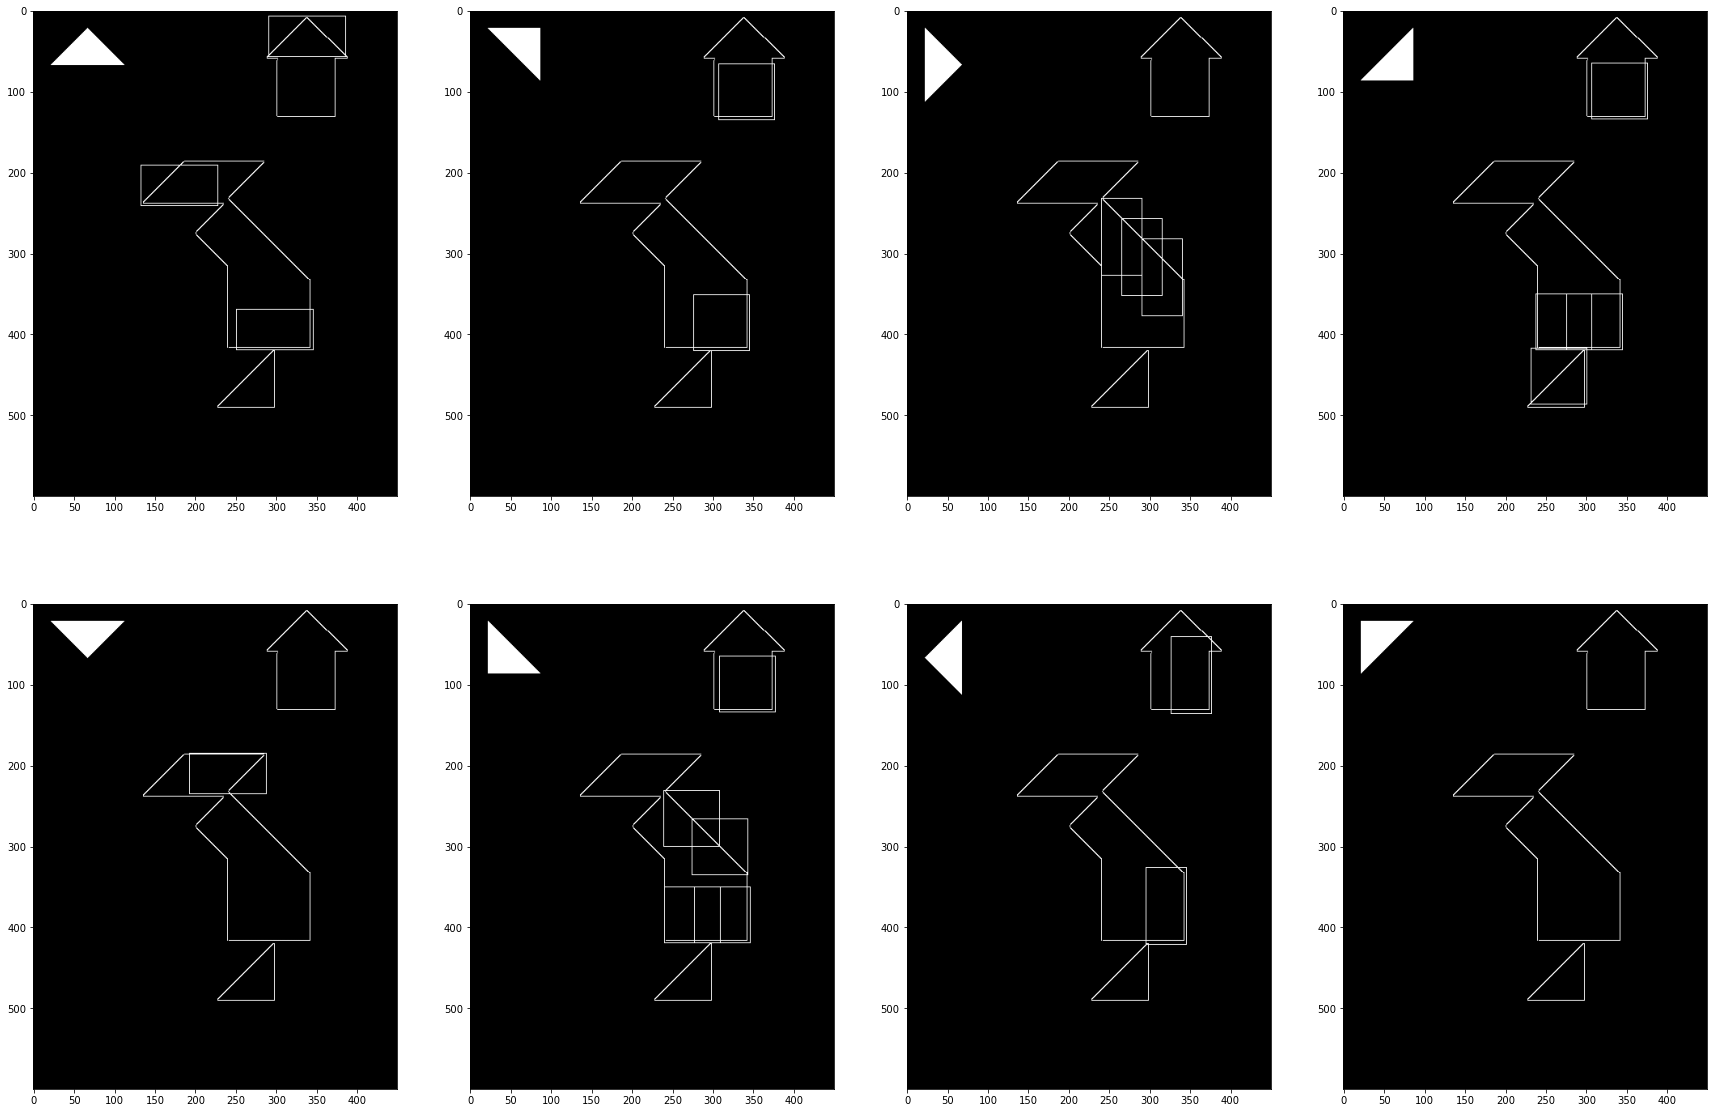
\includegraphics[scale=0.2]{pictures/extracted_no_intersect_1.png}
		\caption[]{Extracted landmarks before intersecting with human data}
		\label{fig:extracted_no_intersect_1}
	\end{figure}
    \\The second screening checks for feasibility: the template matching method applied aims to
    simulate a possible cognitive mechanism, but is in no way plausible per-se and might find
    patterns that are unseen or hardly seen by the humans. As a consequence, only the placements
    that have some representation in the training data at the current phase of the solution are
    kept. This also tackles an additional aspect: once a landmark is found its strength must be
    defined, which in turn will determine the baseline activation of the landmark chunk itself in
    the model. While a possible solution would be basing the strength on the similarity value, this
    would not have any cognitive foundation. \\On the other hand, the data provide a clear indicator
    of its likelihood: if a large number of participants acted on the landmark in the current phase
    of the game, it should in turn mean that such landmark should be a strong landmark. The
    frequency count is thus used not only for screening, but also for defining the baseline
    activation of the chunk once loaded into the declarative memory.\\
    As the human's visual (working?) memory is limited [cite maybe 7+-2, or something more
    relevant], only the 6 strongest landmarks will define the imaginal buffer, with the rest being
    merely loaded into the declarative memory with their respective strength.\\
    A final task performed by the visual system, is to recognize the presence of problematic regions
    (UNF-REGIONS): in principle, such regions are parts of the silhouette in which no tan can be
    placed respecting the rules. They cannot be matched directly as they come in various different
    shapes and sizes, but a property of the task can be exploited to identify some of them: the
    silhouette area must eventually be fully covered and all available pieces used. Considering
    this, if at any point in time no available placement is found for a piece,it means that its area
    is split between two or more separate regions that cannot accommodate it. In such cases, the
    presence of a problematic region is found and the last action is marked as uncertain.
    
    \section{Coordinator}
    The coordinator is the main python application, providing the interfacing features between the
    other modules. It initializes the various sub-components, keeps an internal representation of
    the puzzle state and updates it accordance to the chosen ACT-R action.
    \subsection{State representation}
    The tangram puzzle currently being solved is represented by the eponymous class \textit{Puzzle}.
    Its fields are mainly used for listing the free tans, the currently used tans, their respective
    positioning and the landmarks they are involved in. While in principle the definition of the
    landmark already includes the involved piece, the presence of multiple tans of the same type
    requires such distinction, in order to avoid acting on already placed landmarks. A given action
    is thus defined as a tuple (Piece, Landmark). A list of the overall sequence of actions is
    finally stored for the performance evaluation.
    \subsection{Updating actions}
    While the ACT-R module will provide the reasoning and eventually choose the action performed at
    each step, the implementation of such action is delegated to the coordinator. The main methods
    that provide such functionalities are described in the following:
    \begin{itemize}
        \item \textbf{update}: the update method represents the main operation for the task
        solution. Accepting a landmark definition (piece type, position, orientation) it picks the
        first available piece corresponding to such type, creates the (Piece, Landmark) match, and
        updates the state accordingly.
        \item \textbf{region\_backtrack}: this method ideally represents the attempt for
        backtracking when a region that cannot fit any available piece is identified. Humans (and
        thus the agent) do not necessarily act on such problematic regions in the moment they
        produce them, but only once they are noticed. \\In order to simulate such behaviour, the
        visual system will flag such occurrence as soon as it appears, by creating an "UNF-REGION"
        landmark, but the method will be called only once the agent actually matches it via firing
        the backtracking production. All actions performed while such a landmark exists will be
        flagged as potentially problematic, and every time the method is called, the first such
        action will be backtracked, possibly clearing the queue if the issue is not present anymore.
        \item \textbf{piece\_backtrack}: backtracking can happen even if no problematic region is
        matched: participants can realize that a current placement is leading to no solution, or
        fail to identify a possible landmark. Both of these cases are represented by a retrieval
        failure, which in turn triggers the piece\_backtrack method. \\In this case no information
        about problematic placements is available, so the decision on which action to backtrack is
        based on the landmark strength, as determined by the data. For each of the active landmark
        the function extracts its frequency count at the current game state, and the weakest one is
        chosen for backtracking.
    \end{itemize}
    
    \section{ACT-R model}
	The ACT-R model is tasked with choosing the next action to take at any given position, and it is
	mostly based on the baseline activation and spreading activation mechanisms; three modules are
	involved in the process: the imaginal module, the declarative module and the retrieval module.\\
	As previously described, the visual system extracts the current landmarks, adds them to the
	declarative memory according to their strength, and subsequently loads the 6 strongest into the
	imaginal buffer. In this context, the imaginal buffer represents the "most noticeable"
	landmarks, and helps their retrieval by the spreading activation mechanism.\\
	A description of the main production rules follow:
	\begin{itemize}
	    \item \textbf{retrieve-landmark}: as the name suggests, this production calls for a
	    retrieval of any given landmark. It matches when there are still pieces available and at
	    least one noticed landmark is in the imaginal buffer.It poses no restrictions on the
	    retrieval request, other than asking for a landmark chunk which has not been recently
	    retrieved.\\
	    The retrieval process is then guided by three components: the baseline activation, which is
	    provided at chunk definition (by the visual system) and depends on the landmark strength,
	    the spreading activation, depending on the landmark chunks present in the imaginal buffer,
	    and a noise component, the distribution of which is an hyperparameter of the model.\\
	    \item \textbf{act-and-update}: this production is triggered whenever the retrieval from
	    \textbf{retrieve-landmark} is successful. Its task is to extract the relevant fields from
	    the landmark chunk and to provide them to the coordinator, by calling the \textbf{update}
	    method.\\
	    \item \textbf{fail-to-retrieve}: the experiments additionally show that a participant might
	    fail to retrieve certain landmarks even if they are visible and representing a near
	    "perfect-match". In order to simulate such behaviour, a retrieval threshold value is
	    introduced: if, due to noise or weakness of activation, no landmark's activation is above
	    the threshold a buffer failure will happen in the retrieval request. Such failure is matched
	    by the production \textbf{fail-to-retrieve}, its purpose being to trigger the
	    \textbf{piece\_backtrack} procedure.
	    \item \textbf{notice-problem}: this production is in direct competition with
	    \textbf{retrieve-landmark} whenever the special landmark \textit{UNF-REG} is present in the
	    imaginal buffer. This represents the participant noticing a problematic region in the puzzle
	    and thus starting the backtracking process of solving such region.
	    \item \textbf{solve-problem}: this production directy follows \textbf{notice-problem} and,
	    in a similar fashion to \textbf{fail-to-retrieve}, its task is to interact with the
	    coordinator in order to call the correct backtracking method.\\
	    
	\end{itemize}
	The interaction between the two backtracking procedures should be noted: in some cases, a given
	incorrect placement of a piece does not create any recognizable unfeasible-region, but will
	cause all the following actions to be problematic. This will not be noticed by any of the two
	individual productions, but it will eventually be possible to backtrack by their combination.
	Due to the constraint on \textit{:recently-retrieved nil}, after various iterations of the
	\textbf{region\_backtracking} with no solution, no new landmark will be available. At this point
	the \textbf{piece\_backtracking} method will be triggered, which will remove the weakest
	landmark. At later phases of the solution, the problematic landmarks will be less frequent, as
	more participants will actually have solved the puzzle, and its strength in the model will thus
	be lowered.
  
	
	\chapter{Results and evaluation}
    Where I compare the model to the expected data and try to discuss whether the hypothesis are
    funded and whether there are possible applications
	
	\chapter{Conclusions and future developments}
	\appendix
	
	\printbibliography[heading=bibintoc] % biblatex

	
	\acknowledgements
		
		
\end{document}